% !TEX TS-program = xelatex
% !TEX encoding = UTF-8 Unicode
% !Mode:: "TeX:UTF-8"

\documentclass{resume}
\usepackage{graphicx}
\usepackage{tabu}
\usepackage{tabularx}
\usepackage{multirow}
\usepackage{progressbar}
\usepackage{zh_CN-Adobefonts_external} % Simplified Chinese Support using external fonts (./fonts/zh_CN-Adobe/)
\usepackage{tikz}
% \usepackage{NotoSansSC_external}
% \usepackage{NotoSerifCJKsc_external}
% \usepackage{zh_CN-Adobefonts_internal} % Simplified Chinese Support using system fonts
\usepackage{linespacing_fix} % disable extra space before next section
\usepackage{cite}

\newcommand{\hlink}[1]{\href{#1}{#1}}

\begin{document}
\pagenumbering{gobble} % suppress displaying page number

\medskip\noindent
\begin{minipage}{0.7\textwidth}
  \Large{
    \begin{tabu}  { l }
      \scshape{Tang Zongxun (唐宗勋)} \\
      \email{tangzongxun@hotmail.com} \\
      \phone{(+86) 13070156080} \\
      \linkedin[tangzongxun]{https://www.linkedin.com/in/tangzongxun} \\
    \end{tabu}
  }
\end{minipage}
\begin{minipage}{0.3\textwidth}
  \raggedleft
  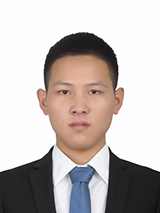
\includegraphics[height=30mm]{me}
\end{minipage}

% \name{唐宗勋}
%
% \basicInfo{
%   \email{tangzongxun@hotmail.com} \textperiodcentered\ 
%   \phone{(+86) 13070156080} \textperiodcentered\ 
%   \linkedin[tangzongxun]{https://www.linkedin.com/in/tangzongxun}}


\section{\faGraduationCap\  Education}
\datedsubsection{\textbf{Beihang University}, Beijing}{2017 -- Now}
\textit{Master's student}\ Electronic and Communication Engineering, Anticipated Graduation: January 2020.
\datedsubsection{\textbf{Beihang University}, Beijing}{2013 -- 2017}
\textit{Bachelor}\ Electronic and Information Engineering.
Top 30\%

\section{\faUsers\ Experiences}
\datedsubsection{\textbf{libsm}}{March 2018 -- July 2018}
\role{Rust}{Cooperate with Cryptape}
A Rust library of Standard Encryption Algorithms of China. \hlink{https://github.com/cryptape/libsm}
\begin{itemize}
  \item As the main author, I implemented hash function, symmetric cipher and digital signature.
  \item This library has been used in CITA(\hlink{https://github.com/cryptape/cita}).
\end{itemize}

\datedsubsection{\textbf{pec-client}}{October 2018 -- December 2019}
\role{JavaScript, React}{lab project}
\begin{onehalfspacing}
Web front-end of a blockchain DApp, \hlink{https://github.com/BH-Open-Blockchain-XLab/pec-client}
\begin{itemize}
  \item This is a single-page app using React/Redux.
  \item I implemented pages of logging in, signing on, transaction query, and transaction submitting.
\end{itemize}
\end{onehalfspacing}


\section{\faCogs\ Skills}
% increase linespacing [parsep=0.5ex]
\begin{itemize}[parsep=0.5ex]
  \item Programming Language: C/C++, Python, JavaScript, Rust
  \item Platform: Linux
  \item Tools: Git, Docker
  \item Domain Knowledge: Cryptography, Web Front-end, Blockchain, Signal Processing, Embedded Devices.
\end{itemize}

\section{\faInfo\ Others}
% increase linespacing [parsep=0.5ex]
\begin{itemize}[parsep=0.5ex]
  \item Languages: English - fluent(CET-6 546), Chinese - native speaker.
\end{itemize}

\end{document}
